\section*{DFS and Connectivity of Graphs}


Recall that the \emph{explore} function starting from a given vertex $v$ finds
all vertices in $G$ reachable from $v$.  Below we give two examples of running $explore$. 
%We represent the running process
%using a \emph{search graph}: 
%we draw a new vertex $v_j$ in the search graph when we start calling $explore~(G, v_j)$; 
%we draw a \emph{tree edge}, shown with solid lines below, if we examine an edge $(v_i, v_j)$ and $visited[j] = 0$;
%we draw a \emph{back edge}, shown with dashed lines below, if we examine an edge $(v_i, v_j)$ and $visited[j] = 1$.

\begin{figure}[h!]
\centering{

\tikzset{every picture/.style={line width=0.75pt}} %set default line width to 0.75pt        

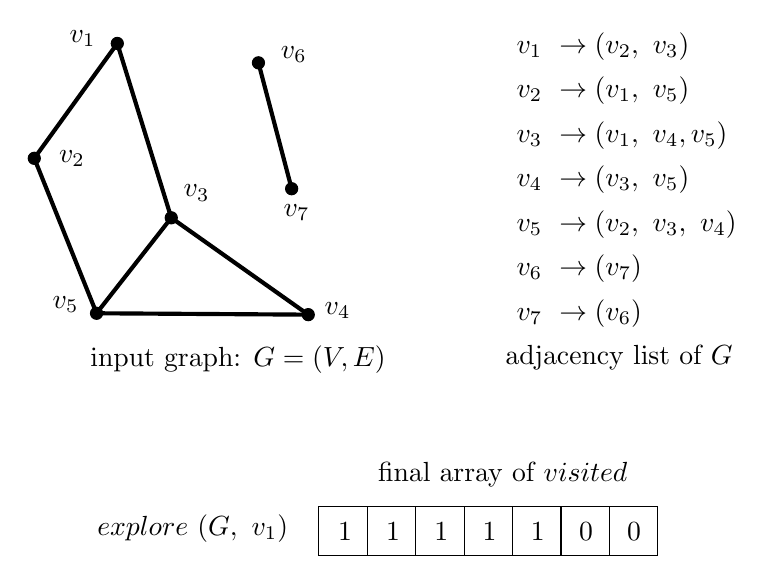
\begin{tikzpicture}[x=0.5pt,y=0.5pt,yscale=-1,xscale=1]
%uncomment if require: \path (0,403); %set diagram left start at 0, and has height of 403

%Flowchart: Connector [id:dp21609803984635512] 
\draw  [fill={rgb, 255:red, 0; green, 0; blue, 0 }  ,fill opacity=1 ] (78,14) .. controls (78,11.58) and (79.96,9.62) .. (82.38,9.62) .. controls (84.79,9.62) and (86.75,11.58) .. (86.75,14) .. controls (86.75,16.42) and (84.79,18.38) .. (82.38,18.38) .. controls (79.96,18.38) and (78,16.42) .. (78,14) -- cycle ;
%Flowchart: Connector [id:dp38532065040165187] 
\draw  [fill={rgb, 255:red, 0; green, 0; blue, 0 }  ,fill opacity=1 ] (180,28) .. controls (180,25.58) and (181.96,23.62) .. (184.38,23.62) .. controls (186.79,23.62) and (188.75,25.58) .. (188.75,28) .. controls (188.75,30.42) and (186.79,32.38) .. (184.38,32.38) .. controls (181.96,32.38) and (180,30.42) .. (180,28) -- cycle ;
%Flowchart: Connector [id:dp39351090897860475] 
\draw  [fill={rgb, 255:red, 0; green, 0; blue, 0 }  ,fill opacity=1 ] (63,209) .. controls (63,206.58) and (64.96,204.62) .. (67.38,204.62) .. controls (69.79,204.62) and (71.75,206.58) .. (71.75,209) .. controls (71.75,211.42) and (69.79,213.38) .. (67.38,213.38) .. controls (64.96,213.38) and (63,211.42) .. (63,209) -- cycle ;
%Flowchart: Connector [id:dp8051888405955012] 
\draw  [fill={rgb, 255:red, 0; green, 0; blue, 0 }  ,fill opacity=1 ] (18,97) .. controls (18,94.58) and (19.96,92.62) .. (22.38,92.62) .. controls (24.79,92.62) and (26.75,94.58) .. (26.75,97) .. controls (26.75,99.42) and (24.79,101.38) .. (22.38,101.38) .. controls (19.96,101.38) and (18,99.42) .. (18,97) -- cycle ;
%Flowchart: Connector [id:dp7816891500218178] 
\draw  [fill={rgb, 255:red, 0; green, 0; blue, 0 }  ,fill opacity=1 ] (117,140) .. controls (117,137.58) and (118.96,135.62) .. (121.38,135.62) .. controls (123.79,135.62) and (125.75,137.58) .. (125.75,140) .. controls (125.75,142.42) and (123.79,144.38) .. (121.38,144.38) .. controls (118.96,144.38) and (117,142.42) .. (117,140) -- cycle ;
%Straight Lines [id:da6208899950626718] 
\draw [color={rgb, 255:red, 0; green, 0; blue, 0 }  ,draw opacity=1 ][line width=1.5]    (22.38,97) -- (82.38,14) ;
%Straight Lines [id:da7339540599990945] 
\draw [color={rgb, 255:red, 0; green, 0; blue, 0 }  ,draw opacity=1 ][line width=1.5]    (67.38,209) -- (121.38,140) ;
%Straight Lines [id:da35316403261996787] 
\draw [color={rgb, 255:red, 0; green, 0; blue, 0 }  ,draw opacity=1 ][line width=1.5]    (121.38,140) -- (82.38,14) ;
%Straight Lines [id:da9584150919133847] 
\draw [color={rgb, 255:red, 0; green, 0; blue, 0 }  ,draw opacity=1 ][line width=1.5]    (67.38,209) -- (22.38,97) ;
%Flowchart: Connector [id:dp23598018985885927] 
\draw  [fill={rgb, 255:red, 0; green, 0; blue, 0 }  ,fill opacity=1 ] (216,210) .. controls (216,207.58) and (217.96,205.62) .. (220.38,205.62) .. controls (222.79,205.62) and (224.75,207.58) .. (224.75,210) .. controls (224.75,212.42) and (222.79,214.38) .. (220.38,214.38) .. controls (217.96,214.38) and (216,212.42) .. (216,210) -- cycle ;
%Straight Lines [id:da22776662357409172] 
\draw [color={rgb, 255:red, 0; green, 0; blue, 0 }  ,draw opacity=1 ][line width=1.5]    (220.38,210) -- (121.38,140) ;
%Straight Lines [id:da7584009034446212] 
\draw [color={rgb, 255:red, 0; green, 0; blue, 0 }  ,draw opacity=1 ][line width=1.5]    (67.38,209) -- (220.38,210) ;
%Flowchart: Connector [id:dp35704899907608434] 
\draw  [fill={rgb, 255:red, 0; green, 0; blue, 0 }  ,fill opacity=1 ] (204,119) .. controls (204,116.58) and (205.96,114.62) .. (208.38,114.62) .. controls (210.79,114.62) and (212.75,116.58) .. (212.75,119) .. controls (212.75,121.42) and (210.79,123.38) .. (208.38,123.38) .. controls (205.96,123.38) and (204,121.42) .. (204,119) -- cycle ;
%Straight Lines [id:da9295589043208872] 
\draw [color={rgb, 255:red, 0; green, 0; blue, 0 }  ,draw opacity=1 ][line width=1.5]    (208.38,119) -- (184.38,28) ;
%Shape: Grid [id:dp7483322939455812] 
\draw  [draw opacity=0] (228,348.87) -- (473,348.87) -- (473,383.87) -- (228,383.87) -- cycle ; \draw   (263,348.87) -- (263,383.87)(298,348.87) -- (298,383.87)(333,348.87) -- (333,383.87)(368,348.87) -- (368,383.87)(403,348.87) -- (403,383.87)(438,348.87) -- (438,383.87) ; \draw    ; \draw   (228,348.87) -- (473,348.87) -- (473,383.87) -- (228,383.87) -- cycle ;

% Text Node
\draw (46,3) node [anchor=north west][inner sep=0.75pt]   [align=left] {$\displaystyle v_{1}$};
% Text Node
\draw (128.38,114.38) node [anchor=north west][inner sep=0.75pt]   [align=left] {$\displaystyle v_{3}$};
% Text Node
\draw (33.75,195) node [anchor=north west][inner sep=0.75pt]   [align=left] {$\displaystyle v_{5}$};
% Text Node
\draw (230.38,199.38) node [anchor=north west][inner sep=0.75pt]   [align=left] {$\displaystyle v_{4}$};
% Text Node
\draw (38.38,89.38) node [anchor=north west][inner sep=0.75pt]   [align=left] {$\displaystyle v_{2}$};
% Text Node
\draw (369,4.09) node [anchor=north west][inner sep=0.75pt]   [align=left] {$\displaystyle v_{1} \ \rightarrow ( v_{2} ,\ v_{3})$};
% Text Node
\draw (369,36.26) node [anchor=north west][inner sep=0.75pt]   [align=left] {$\displaystyle v_{2} \ \rightarrow ( v_{1} ,\ v_{5})$};
% Text Node
\draw (369,68.43) node [anchor=north west][inner sep=0.75pt]   [align=left] {$\displaystyle v_{3} \ \rightarrow ( v_{1} ,\ v_{4} ,v_{5})$};
% Text Node
\draw (369,100.6) node [anchor=north west][inner sep=0.75pt]   [align=left] {$\displaystyle v_{4} \ \rightarrow ( v_{3} ,\ v_{5})$ \ };
% Text Node
\draw (369,132.77) node [anchor=north west][inner sep=0.75pt]   [align=left] {$\displaystyle v_{5} \ \rightarrow ( v_{2} ,\ v_{3} ,\ v_{4})$};
% Text Node
\draw (198.75,14.35) node [anchor=north west][inner sep=0.75pt]   [align=left] {$\displaystyle v_{6}$};
% Text Node
\draw (200.75,128.35) node [anchor=north west][inner sep=0.75pt]   [align=left] {$\displaystyle v_{7}$};
% Text Node
\draw (369,164.94) node [anchor=north west][inner sep=0.75pt]   [align=left] {$\displaystyle v_{6} \ \rightarrow ( v_{7})$ \ };
% Text Node
\draw (369,197.09) node [anchor=north west][inner sep=0.75pt]   [align=left] {$\displaystyle v_{7} \ \rightarrow ( v_{6})$};
% Text Node
\draw (61,230.93) node [anchor=north west][inner sep=0.75pt]   [align=left] {input graph: $\displaystyle G=( V,E)$};
% Text Node
\draw (361,229.93) node [anchor=north west][inner sep=0.75pt]   [align=left] {adjacency list of $\displaystyle G$};
% Text Node
\draw (66,352.93) node [anchor=north west][inner sep=0.75pt]   [align=left] { $\displaystyle explore\ ( G,\ v_{1})$};
% Text Node
\draw (269,314.93) node [anchor=north west][inner sep=0.75pt]   [align=left] {final array of $\displaystyle visited$};
% Text Node
\draw (240,358.37) node [anchor=north west][inner sep=0.75pt]   [align=left] {$\displaystyle 1$};
% Text Node
\draw (274.83,358.37) node [anchor=north west][inner sep=0.75pt]   [align=left] {$\displaystyle 1$};
% Text Node
\draw (309.66,358.37) node [anchor=north west][inner sep=0.75pt]   [align=left] {$\displaystyle 1$};
% Text Node
\draw (344.49,358.37) node [anchor=north west][inner sep=0.75pt]   [align=left] {$\displaystyle 1$};
% Text Node
\draw (379.32,358.37) node [anchor=north west][inner sep=0.75pt]   [align=left] {$\displaystyle 1$};
% Text Node
\draw (414.15,358.37) node [anchor=north west][inner sep=0.75pt]   [align=left] {$\displaystyle 0$};
% Text Node
\draw (449,358.37) node [anchor=north west][inner sep=0.75pt]   [align=left] {$\displaystyle 0$};


\end{tikzpicture}

}
\caption{Running $explore~(G, v_1)$ on an undirected graph.}
\label{fig:explore-undirected}
\end{figure}

\begin{figure}[h!]
\centering{

\tikzset{every picture/.style={line width=0.75pt}} %set default line width to 0.75pt        

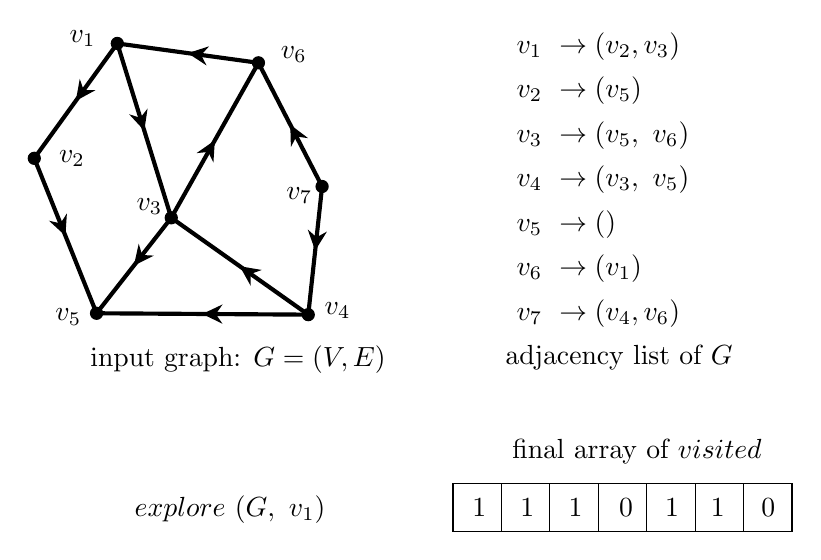
\begin{tikzpicture}[x=0.5pt,y=0.5pt,yscale=-1,xscale=1]
%uncomment if require: \path (0,383); %set diagram left start at 0, and has height of 383

%Flowchart: Connector [id:dp036501097648878655] 
\draw  [fill={rgb, 255:red, 0; green, 0; blue, 0 }  ,fill opacity=1 ] (78,14) .. controls (78,11.58) and (79.96,9.62) .. (82.38,9.62) .. controls (84.79,9.62) and (86.75,11.58) .. (86.75,14) .. controls (86.75,16.42) and (84.79,18.38) .. (82.38,18.38) .. controls (79.96,18.38) and (78,16.42) .. (78,14) -- cycle ;
%Flowchart: Connector [id:dp9052812520624474] 
\draw  [fill={rgb, 255:red, 0; green, 0; blue, 0 }  ,fill opacity=1 ] (180,28) .. controls (180,25.58) and (181.96,23.62) .. (184.38,23.62) .. controls (186.79,23.62) and (188.75,25.58) .. (188.75,28) .. controls (188.75,30.42) and (186.79,32.38) .. (184.38,32.38) .. controls (181.96,32.38) and (180,30.42) .. (180,28) -- cycle ;
%Flowchart: Connector [id:dp6707473558764397] 
\draw  [fill={rgb, 255:red, 0; green, 0; blue, 0 }  ,fill opacity=1 ] (63,209) .. controls (63,206.58) and (64.96,204.62) .. (67.38,204.62) .. controls (69.79,204.62) and (71.75,206.58) .. (71.75,209) .. controls (71.75,211.42) and (69.79,213.38) .. (67.38,213.38) .. controls (64.96,213.38) and (63,211.42) .. (63,209) -- cycle ;
%Flowchart: Connector [id:dp21324460835750736] 
\draw  [fill={rgb, 255:red, 0; green, 0; blue, 0 }  ,fill opacity=1 ] (18,97) .. controls (18,94.58) and (19.96,92.62) .. (22.38,92.62) .. controls (24.79,92.62) and (26.75,94.58) .. (26.75,97) .. controls (26.75,99.42) and (24.79,101.38) .. (22.38,101.38) .. controls (19.96,101.38) and (18,99.42) .. (18,97) -- cycle ;
%Flowchart: Connector [id:dp1646273807568044] 
\draw  [fill={rgb, 255:red, 0; green, 0; blue, 0 }  ,fill opacity=1 ] (117,140) .. controls (117,137.58) and (118.96,135.62) .. (121.38,135.62) .. controls (123.79,135.62) and (125.75,137.58) .. (125.75,140) .. controls (125.75,142.42) and (123.79,144.38) .. (121.38,144.38) .. controls (118.96,144.38) and (117,142.42) .. (117,140) -- cycle ;
%Straight Lines [id:da7734477732656454] 
\draw [color={rgb, 255:red, 0; green, 0; blue, 0 }  ,draw opacity=1 ][line width=1.5]    (22.38,97) -- (82.38,14) ;
\draw [shift={(52.38,55.5)}, rotate = 305.86] [fill={rgb, 255:red, 0; green, 0; blue, 0 }  ,fill opacity=1 ][line width=0.08]  [draw opacity=0] (14.56,-6.99) -- (0,0) -- (14.56,6.99) -- (9.67,0) -- cycle    ;
%Straight Lines [id:da04451412587827308] 
\draw [color={rgb, 255:red, 0; green, 0; blue, 0 }  ,draw opacity=1 ][line width=1.5]    (67.38,209) -- (121.38,140) ;
\draw [shift={(94.38,174.5)}, rotate = 308.05] [fill={rgb, 255:red, 0; green, 0; blue, 0 }  ,fill opacity=1 ][line width=0.08]  [draw opacity=0] (14.56,-6.99) -- (0,0) -- (14.56,6.99) -- (9.67,0) -- cycle    ;
%Straight Lines [id:da2600695048882036] 
\draw [color={rgb, 255:red, 0; green, 0; blue, 0 }  ,draw opacity=1 ][line width=1.5]    (121.38,140) -- (82.38,14) ;
\draw [shift={(101.88,77)}, rotate = 252.8] [fill={rgb, 255:red, 0; green, 0; blue, 0 }  ,fill opacity=1 ][line width=0.08]  [draw opacity=0] (14.56,-6.99) -- (0,0) -- (14.56,6.99) -- (9.67,0) -- cycle    ;
%Straight Lines [id:da6431378909446039] 
\draw [color={rgb, 255:red, 0; green, 0; blue, 0 }  ,draw opacity=1 ][line width=1.5]    (67.38,209) -- (22.38,97) ;
\draw [shift={(44.88,153)}, rotate = 248.11] [fill={rgb, 255:red, 0; green, 0; blue, 0 }  ,fill opacity=1 ][line width=0.08]  [draw opacity=0] (14.56,-6.99) -- (0,0) -- (14.56,6.99) -- (9.67,0) -- cycle    ;
%Flowchart: Connector [id:dp5116336083980441] 
\draw  [fill={rgb, 255:red, 0; green, 0; blue, 0 }  ,fill opacity=1 ] (216,210) .. controls (216,207.58) and (217.96,205.62) .. (220.38,205.62) .. controls (222.79,205.62) and (224.75,207.58) .. (224.75,210) .. controls (224.75,212.42) and (222.79,214.38) .. (220.38,214.38) .. controls (217.96,214.38) and (216,212.42) .. (216,210) -- cycle ;
%Straight Lines [id:da2162845882048139] 
\draw [color={rgb, 255:red, 0; green, 0; blue, 0 }  ,draw opacity=1 ][line width=1.5]    (220.38,210) -- (121.38,140) ;
\draw [shift={(170.88,175)}, rotate = 35.26] [fill={rgb, 255:red, 0; green, 0; blue, 0 }  ,fill opacity=1 ][line width=0.08]  [draw opacity=0] (14.56,-6.99) -- (0,0) -- (14.56,6.99) -- (9.67,0) -- cycle    ;
%Straight Lines [id:da5227829916512413] 
\draw [color={rgb, 255:red, 0; green, 0; blue, 0 }  ,draw opacity=1 ][line width=1.5]    (67.38,209) -- (220.38,210) ;
\draw [shift={(143.88,209.5)}, rotate = 0.37] [fill={rgb, 255:red, 0; green, 0; blue, 0 }  ,fill opacity=1 ][line width=0.08]  [draw opacity=0] (14.56,-6.99) -- (0,0) -- (14.56,6.99) -- (9.67,0) -- cycle    ;
%Flowchart: Connector [id:dp35238628980993314] 
\draw  [fill={rgb, 255:red, 0; green, 0; blue, 0 }  ,fill opacity=1 ] (226,117.38) .. controls (226,114.96) and (227.96,113) .. (230.38,113) .. controls (232.79,113) and (234.75,114.96) .. (234.75,117.38) .. controls (234.75,119.79) and (232.79,121.75) .. (230.38,121.75) .. controls (227.96,121.75) and (226,119.79) .. (226,117.38) -- cycle ;
%Straight Lines [id:da9207154473288715] 
\draw [color={rgb, 255:red, 0; green, 0; blue, 0 }  ,draw opacity=1 ][line width=1.5]    (230.38,117.38) -- (184.38,28) ;
\draw [shift={(207.38,72.69)}, rotate = 62.77] [fill={rgb, 255:red, 0; green, 0; blue, 0 }  ,fill opacity=1 ][line width=0.08]  [draw opacity=0] (14.56,-6.99) -- (0,0) -- (14.56,6.99) -- (9.67,0) -- cycle    ;
%Shape: Grid [id:dp00896828173959141] 
\draw  [draw opacity=0] (325,331.87) -- (570,331.87) -- (570,366.87) -- (325,366.87) -- cycle ; \draw   (360,331.87) -- (360,366.87)(395,331.87) -- (395,366.87)(430,331.87) -- (430,366.87)(465,331.87) -- (465,366.87)(500,331.87) -- (500,366.87)(535,331.87) -- (535,366.87) ; \draw    ; \draw   (325,331.87) -- (570,331.87) -- (570,366.87) -- (325,366.87) -- cycle ;
%Straight Lines [id:da419452024727319] 
\draw [color={rgb, 255:red, 0; green, 0; blue, 0 }  ,draw opacity=1 ][line width=1.5]    (121.38,140) -- (184.38,28) ;
\draw [shift={(152.88,84)}, rotate = 119.36] [fill={rgb, 255:red, 0; green, 0; blue, 0 }  ,fill opacity=1 ][line width=0.08]  [draw opacity=0] (14.56,-6.99) -- (0,0) -- (14.56,6.99) -- (9.67,0) -- cycle    ;
%Straight Lines [id:da9548831345515606] 
\draw [color={rgb, 255:red, 0; green, 0; blue, 0 }  ,draw opacity=1 ][line width=1.5]    (82.38,14) -- (184.38,28) ;
\draw [shift={(133.38,21)}, rotate = 7.82] [fill={rgb, 255:red, 0; green, 0; blue, 0 }  ,fill opacity=1 ][line width=0.08]  [draw opacity=0] (14.56,-6.99) -- (0,0) -- (14.56,6.99) -- (9.67,0) -- cycle    ;
%Straight Lines [id:da2533545377621541] 
\draw [color={rgb, 255:red, 0; green, 0; blue, 0 }  ,draw opacity=1 ][line width=1.5]    (220.38,210) -- (230.38,117.38) ;
\draw [shift={(225.38,163.69)}, rotate = 276.16] [fill={rgb, 255:red, 0; green, 0; blue, 0 }  ,fill opacity=1 ][line width=0.08]  [draw opacity=0] (14.56,-6.99) -- (0,0) -- (14.56,6.99) -- (9.67,0) -- cycle    ;

% Text Node
\draw (46,3) node [anchor=north west][inner sep=0.75pt]   [align=left] {$\displaystyle v_{1}$};
% Text Node
\draw (94.38,124.38) node [anchor=north west][inner sep=0.75pt]   [align=left] {$\displaystyle v_{3}$};
% Text Node
\draw (35.75,204) node [anchor=north west][inner sep=0.75pt]   [align=left] {$\displaystyle v_{5}$};
% Text Node
\draw (230.38,199.38) node [anchor=north west][inner sep=0.75pt]   [align=left] {$\displaystyle v_{4}$};
% Text Node
\draw (38.38,89.38) node [anchor=north west][inner sep=0.75pt]   [align=left] {$\displaystyle v_{2}$};
% Text Node
\draw (369,4.09) node [anchor=north west][inner sep=0.75pt]   [align=left] {$\displaystyle v_{1} \ \rightarrow ( v_{2} ,v_{3})$};
% Text Node
\draw (369,36.26) node [anchor=north west][inner sep=0.75pt]   [align=left] {$\displaystyle v_{2} \ \rightarrow ( v_{5})$};
% Text Node
\draw (369,68.43) node [anchor=north west][inner sep=0.75pt]   [align=left] {$\displaystyle v_{3} \ \rightarrow ( v_{5} ,\ v_{6})$};
% Text Node
\draw (369,100.6) node [anchor=north west][inner sep=0.75pt]   [align=left] {$\displaystyle v_{4} \ \rightarrow ( v_{3} ,\ v_{5})$ \ };
% Text Node
\draw (369,132.77) node [anchor=north west][inner sep=0.75pt]   [align=left] {$\displaystyle v_{5} \ \rightarrow ()$};
% Text Node
\draw (198.75,14.35) node [anchor=north west][inner sep=0.75pt]   [align=left] {$\displaystyle v_{6}$};
% Text Node
\draw (202.75,116.35) node [anchor=north west][inner sep=0.75pt]   [align=left] {$\displaystyle v_{7}$};
% Text Node
\draw (369,164.94) node [anchor=north west][inner sep=0.75pt]   [align=left] {$\displaystyle v_{6} \ \rightarrow ( v_{1} )$ \ };
% Text Node
\draw (369,197.09) node [anchor=north west][inner sep=0.75pt]   [align=left] {$\displaystyle v_{7} \ \rightarrow ( v_{4} ,v_{6})$};
% Text Node
\draw (61,230.93) node [anchor=north west][inner sep=0.75pt]   [align=left] {input graph: $\displaystyle G=( V,E)$};
% Text Node
\draw (361,229.93) node [anchor=north west][inner sep=0.75pt]   [align=left] {adjacency list of $\displaystyle G$};
% Text Node
\draw (93,338.93) node [anchor=north west][inner sep=0.75pt]   [align=left] {$\displaystyle explore\ ( G,\ v_{1})$};
% Text Node
\draw (366,297.93) node [anchor=north west][inner sep=0.75pt]   [align=left] {final array of $\displaystyle visited$};
% Text Node
\draw (337,341.37) node [anchor=north west][inner sep=0.75pt]   [align=left] {$\displaystyle 1$};
% Text Node
\draw (371.83,341.37) node [anchor=north west][inner sep=0.75pt]   [align=left] {$\displaystyle 1$};
% Text Node
\draw (406.66,341.37) node [anchor=north west][inner sep=0.75pt]   [align=left] {$\displaystyle 1$};
% Text Node
\draw (509.49,341.37) node [anchor=north west][inner sep=0.75pt]   [align=left] {$\displaystyle 1$};
% Text Node
\draw (476.32,341.37) node [anchor=north west][inner sep=0.75pt]   [align=left] {$\displaystyle 1$};
% Text Node
\draw (443.15,341.37) node [anchor=north west][inner sep=0.75pt]   [align=left] {$\displaystyle 0$};
% Text Node
\draw (546,341.37) node [anchor=north west][inner sep=0.75pt]   [align=left] {$\displaystyle 0$};


\end{tikzpicture}

}
\caption{Running $explore~(G, v_1)$ on an directed graph.}
\label{fig:explore-directed}
\end{figure}

We now define ``connected'' and ``connected component'' to formally reveal the connectivity-structure of graphs.
Let $u,v\in V$. We say $u$ and $v$ are \emph{connected} if and only if there exists a path from $u$ to $v$
\emph{and} there exists a path from $v$ to $u$. 
We note that this definition applies to both directed and undirected graph.
In undirected graph, the existence of a path from $u$ to $v$ implies the
existence of a path from $v$ to $u$. However, this is not necessarily true in directed
graphs. For example, in Figure~\ref{fig:explore-directed}, there exists a path from $v_1$ to $v_5$ but there is no path
from $v_5$ to $v_1$~(so they are not connected).

Let $G = (V, E)$. Let $V_1\subset V$. We say $V_1$ is a \emph{connected component} of $G$,
if and only if (1), for \emph{every pair of} $u,v\in V_1$, $u$ and $v$ are connected,
and (2), $V_1$ is \emph{maximal}, i.e., there does not exists vertex $w\in V\setminus V_1$ such
that $V_1\cup \{w\}$ satisfies condition (1).
For example, in Figure~\ref{fig:explore-directed}, $\{v_1, v_3, v_6\}$ is a connected component;
$\{v_2\}$ is a connected component; 
$\{v_1, v_3\}$ is not a connected component~(as it is not maximal, i.e., does not satisfy condition 2). 

The explore algorithm identifies all vertices that can be reached from $v_i$.
Hence, in the case of undirected graphs, these vertices~(including $v_i$) are pairwise reachable, 
i.e., they form a connected component of $G$~(summarized below). In other words,
$explore(G,v_i)$ identifies the connected component of $G$ that includes $v_i$.

\begin{fact}
For undirected graphs, after $explore(G, v_i)$, the vertices that are marked by $visited$, i.e.,
$\{v_j \mid visited[j] = 1\}$ forms a connected component of $G$ that includes $v_i$.
\end{fact}

However, the above fact does not apply to directed graph: Figure~\ref{fig:explore-directed} gives such an example,
where $\{v_1,v_2,v_3,v_5,v_6\}$ does not form a connected component. Note: in directed graphs
$\{v_j \mid visited[j] = 1\}$ are still those vertices that are reachable from $v_i$; it's just that
they may not be a connected component of $G$.

How to identify \emph{all} connected components of an undirected graph?
We can run above explore algorithm multiple times, each of which starts from an un-explored vertex,
until all vertices are explored. To keep track of which vertices are in which connected
component, we will introduce variable \emph{num-cc} to store the index of current connected component.
We redefine the behavior of $visited$ array: $visited[j] = 0$ still represents that $v_j$ has not yet been explored;
$visited[j] = k$, $k\ge 1$, represents that $v_j$ has been explored and $v_j$ is in the $k$-th connected component.

This new algorithm that traverses all vertices and edges of a graph is named as DFS~(depth first search).
We also slightly changed the explore function, which allows to store which connected component each vertex is in.
The pseudo-codes are given below.

\begin{minipage}{0.8\textwidth}
	\aaA {9}{function DFS ($G = (V, E)$)}\xxx
	\aab {num-cc = 0;}\xxx
	\aab {$visited[i] = 0$, for all $1\le i \le |V|$;}\xxx
	\aaB {5}{for $i = 1 \to |V|$}\xxx
	\aaC {3}{if ($visited[i] = 0$)}\xxx
	\aad {num-cc = num-cc + 1;}\xxx
	\aad {explore ($G, v_i$);}\xxx
	\aac {end if;}\xxx
	\aab {end for;}\xxx
	\aaa {end algorithm;}\xxx
\end{minipage}


\begin{minipage}{0.8\textwidth}
	\aaA {5}{function explore ($G = (V, E), v_i \in V$)}\xxx
	\aab {$visited[i] = $ num-cc;}\xxx
	\aaB {2}{for any edge $(v_i, v_j) \in E$}\xxx
	\aac {if ($visited[j] = 0$): explore ($G, v_j$);}\xxx
	\aab {end for;}\xxx
	\aaa {end algorithm;}\xxx
\end{minipage}

Below we gave examples of running DFS on undirected graphs and undirected graphs.

\begin{figure}[h!]
\centering{

\tikzset{every picture/.style={line width=0.75pt}} %set default line width to 0.75pt        

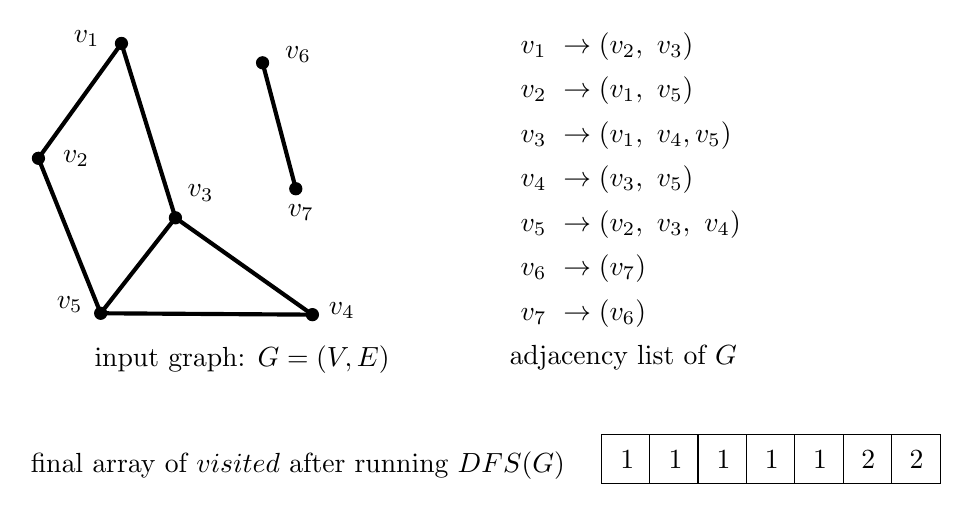
\begin{tikzpicture}[x=0.5pt,y=0.5pt,yscale=-1,xscale=1]
%uncomment if require: \path (0,353); %set diagram left start at 0, and has height of 353

%Flowchart: Connector [id:dp8937679142558405] 
\draw  [fill={rgb, 255:red, 0; green, 0; blue, 0 }  ,fill opacity=1 ] (78,14) .. controls (78,11.58) and (79.96,9.62) .. (82.38,9.62) .. controls (84.79,9.62) and (86.75,11.58) .. (86.75,14) .. controls (86.75,16.42) and (84.79,18.38) .. (82.38,18.38) .. controls (79.96,18.38) and (78,16.42) .. (78,14) -- cycle ;
%Flowchart: Connector [id:dp784072905480598] 
\draw  [fill={rgb, 255:red, 0; green, 0; blue, 0 }  ,fill opacity=1 ] (180,28) .. controls (180,25.58) and (181.96,23.62) .. (184.38,23.62) .. controls (186.79,23.62) and (188.75,25.58) .. (188.75,28) .. controls (188.75,30.42) and (186.79,32.38) .. (184.38,32.38) .. controls (181.96,32.38) and (180,30.42) .. (180,28) -- cycle ;
%Flowchart: Connector [id:dp022772254721651897] 
\draw  [fill={rgb, 255:red, 0; green, 0; blue, 0 }  ,fill opacity=1 ] (63,209) .. controls (63,206.58) and (64.96,204.62) .. (67.38,204.62) .. controls (69.79,204.62) and (71.75,206.58) .. (71.75,209) .. controls (71.75,211.42) and (69.79,213.38) .. (67.38,213.38) .. controls (64.96,213.38) and (63,211.42) .. (63,209) -- cycle ;
%Flowchart: Connector [id:dp49543195835367104] 
\draw  [fill={rgb, 255:red, 0; green, 0; blue, 0 }  ,fill opacity=1 ] (18,97) .. controls (18,94.58) and (19.96,92.62) .. (22.38,92.62) .. controls (24.79,92.62) and (26.75,94.58) .. (26.75,97) .. controls (26.75,99.42) and (24.79,101.38) .. (22.38,101.38) .. controls (19.96,101.38) and (18,99.42) .. (18,97) -- cycle ;
%Flowchart: Connector [id:dp9515784775019982] 
\draw  [fill={rgb, 255:red, 0; green, 0; blue, 0 }  ,fill opacity=1 ] (117,140) .. controls (117,137.58) and (118.96,135.62) .. (121.38,135.62) .. controls (123.79,135.62) and (125.75,137.58) .. (125.75,140) .. controls (125.75,142.42) and (123.79,144.38) .. (121.38,144.38) .. controls (118.96,144.38) and (117,142.42) .. (117,140) -- cycle ;
%Straight Lines [id:da9838237754489216] 
\draw [color={rgb, 255:red, 0; green, 0; blue, 0 }  ,draw opacity=1 ][line width=1.5]    (22.38,97) -- (82.38,14) ;
%Straight Lines [id:da9653235980831391] 
\draw [color={rgb, 255:red, 0; green, 0; blue, 0 }  ,draw opacity=1 ][line width=1.5]    (67.38,209) -- (121.38,140) ;
%Straight Lines [id:da9798242054041456] 
\draw [color={rgb, 255:red, 0; green, 0; blue, 0 }  ,draw opacity=1 ][line width=1.5]    (121.38,140) -- (82.38,14) ;
%Straight Lines [id:da7975395810717695] 
\draw [color={rgb, 255:red, 0; green, 0; blue, 0 }  ,draw opacity=1 ][line width=1.5]    (67.38,209) -- (22.38,97) ;
%Flowchart: Connector [id:dp5597560660362859] 
\draw  [fill={rgb, 255:red, 0; green, 0; blue, 0 }  ,fill opacity=1 ] (216,210) .. controls (216,207.58) and (217.96,205.62) .. (220.38,205.62) .. controls (222.79,205.62) and (224.75,207.58) .. (224.75,210) .. controls (224.75,212.42) and (222.79,214.38) .. (220.38,214.38) .. controls (217.96,214.38) and (216,212.42) .. (216,210) -- cycle ;
%Straight Lines [id:da7311433198213012] 
\draw [color={rgb, 255:red, 0; green, 0; blue, 0 }  ,draw opacity=1 ][line width=1.5]    (220.38,210) -- (121.38,140) ;
%Straight Lines [id:da36451088695440814] 
\draw [color={rgb, 255:red, 0; green, 0; blue, 0 }  ,draw opacity=1 ][line width=1.5]    (67.38,209) -- (220.38,210) ;
%Flowchart: Connector [id:dp4274826720632955] 
\draw  [fill={rgb, 255:red, 0; green, 0; blue, 0 }  ,fill opacity=1 ] (204,119) .. controls (204,116.58) and (205.96,114.62) .. (208.38,114.62) .. controls (210.79,114.62) and (212.75,116.58) .. (212.75,119) .. controls (212.75,121.42) and (210.79,123.38) .. (208.38,123.38) .. controls (205.96,123.38) and (204,121.42) .. (204,119) -- cycle ;
%Straight Lines [id:da8734113512633482] 
\draw [color={rgb, 255:red, 0; green, 0; blue, 0 }  ,draw opacity=1 ][line width=1.5]    (208.38,119) -- (184.38,28) ;
%Shape: Grid [id:dp9526360318390427] 
\draw  [draw opacity=0] (429,296.87) -- (674,296.87) -- (674,331.87) -- (429,331.87) -- cycle ; \draw   (464,296.87) -- (464,331.87)(499,296.87) -- (499,331.87)(534,296.87) -- (534,331.87)(569,296.87) -- (569,331.87)(604,296.87) -- (604,331.87)(639,296.87) -- (639,331.87) ; \draw    ; \draw   (429,296.87) -- (674,296.87) -- (674,331.87) -- (429,331.87) -- cycle ;

% Text Node
\draw (46,3) node [anchor=north west][inner sep=0.75pt]   [align=left] {$\displaystyle v_{1}$};
% Text Node
\draw (128.38,114.38) node [anchor=north west][inner sep=0.75pt]   [align=left] {$\displaystyle v_{3}$};
% Text Node
\draw (33.75,195) node [anchor=north west][inner sep=0.75pt]   [align=left] {$\displaystyle v_{5}$};
% Text Node
\draw (230.38,199.38) node [anchor=north west][inner sep=0.75pt]   [align=left] {$\displaystyle v_{4}$};
% Text Node
\draw (38.38,89.38) node [anchor=north west][inner sep=0.75pt]   [align=left] {$\displaystyle v_{2}$};
% Text Node
\draw (369,4.09) node [anchor=north west][inner sep=0.75pt]   [align=left] {$\displaystyle v_{1} \ \rightarrow ( v_{2} ,\ v_{3})$};
% Text Node
\draw (369,36.26) node [anchor=north west][inner sep=0.75pt]   [align=left] {$\displaystyle v_{2} \ \rightarrow ( v_{1} ,\ v_{5})$};
% Text Node
\draw (369,68.43) node [anchor=north west][inner sep=0.75pt]   [align=left] {$\displaystyle v_{3} \ \rightarrow ( v_{1} ,\ v_{4} ,v_{5})$};
% Text Node
\draw (369,100.6) node [anchor=north west][inner sep=0.75pt]   [align=left] {$\displaystyle v_{4} \ \rightarrow ( v_{3} ,\ v_{5})$ \ };
% Text Node
\draw (369,132.77) node [anchor=north west][inner sep=0.75pt]   [align=left] {$\displaystyle v_{5} \ \rightarrow ( v_{2} ,\ v_{3} ,\ v_{4})$};
% Text Node
\draw (198.75,14.35) node [anchor=north west][inner sep=0.75pt]   [align=left] {$\displaystyle v_{6}$};
% Text Node
\draw (200.75,128.35) node [anchor=north west][inner sep=0.75pt]   [align=left] {$\displaystyle v_{7}$};
% Text Node
\draw (369,164.94) node [anchor=north west][inner sep=0.75pt]   [align=left] {$\displaystyle v_{6} \ \rightarrow ( v_{7})$ \ };
% Text Node
\draw (369,197.09) node [anchor=north west][inner sep=0.75pt]   [align=left] {$\displaystyle v_{7} \ \rightarrow ( v_{6})$};
% Text Node
\draw (61,230.93) node [anchor=north west][inner sep=0.75pt]   [align=left] {input graph: $\displaystyle G=( V,E)$};
% Text Node
\draw (361,229.93) node [anchor=north west][inner sep=0.75pt]   [align=left] {adjacency list of $\displaystyle G$};
% Text Node
\draw (15,306.93) node [anchor=north west][inner sep=0.75pt]   [align=left] {final array of $\displaystyle visited$ after running $\displaystyle DFS( G)$};
% Text Node
\draw (441,306.37) node [anchor=north west][inner sep=0.75pt]   [align=left] {$\displaystyle 1$};
% Text Node
\draw (475.83,306.37) node [anchor=north west][inner sep=0.75pt]   [align=left] {$\displaystyle 1$};
% Text Node
\draw (510.66,306.37) node [anchor=north west][inner sep=0.75pt]   [align=left] {$\displaystyle 1$};
% Text Node
\draw (545.49,306.37) node [anchor=north west][inner sep=0.75pt]   [align=left] {$\displaystyle 1$};
% Text Node
\draw (580.32,306.37) node [anchor=north west][inner sep=0.75pt]   [align=left] {$\displaystyle 1$};
% Text Node
\draw (615.15,306.37) node [anchor=north west][inner sep=0.75pt]   [align=left] {$\displaystyle 2$};
% Text Node
\draw (650,306.37) node [anchor=north west][inner sep=0.75pt]   [align=left] {$\displaystyle 2$};


\end{tikzpicture}

}
\caption{Running $DFS~(G)$ on an undirected graph.}
\label{fig:dfs-undirected}
\end{figure}

\begin{figure}[h!]
\centering{

\tikzset{every picture/.style={line width=0.75pt}} %set default line width to 0.75pt        

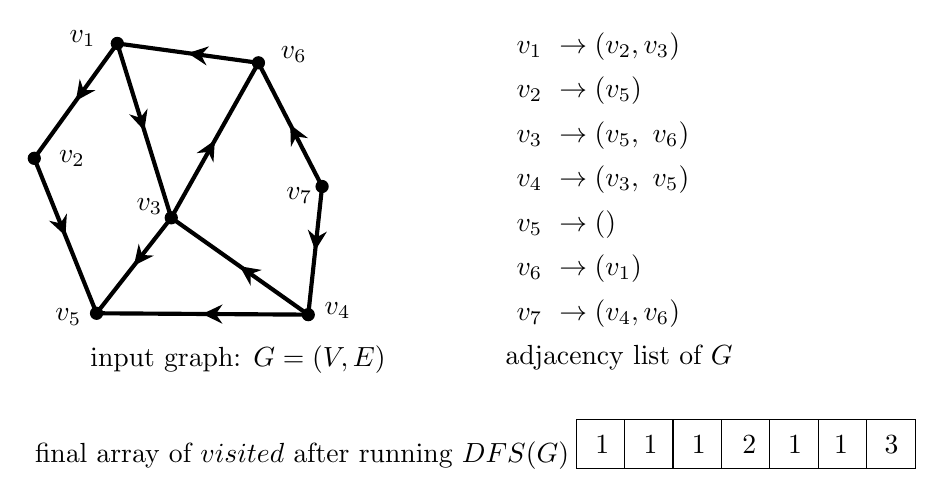
\begin{tikzpicture}[x=0.5pt,y=0.5pt,yscale=-1,xscale=1]
%uncomment if require: \path (0,342); %set diagram left start at 0, and has height of 342

%Flowchart: Connector [id:dp9968125919431555] 
\draw  [fill={rgb, 255:red, 0; green, 0; blue, 0 }  ,fill opacity=1 ] (78,14) .. controls (78,11.58) and (79.96,9.62) .. (82.38,9.62) .. controls (84.79,9.62) and (86.75,11.58) .. (86.75,14) .. controls (86.75,16.42) and (84.79,18.38) .. (82.38,18.38) .. controls (79.96,18.38) and (78,16.42) .. (78,14) -- cycle ;
%Flowchart: Connector [id:dp31888007270335605] 
\draw  [fill={rgb, 255:red, 0; green, 0; blue, 0 }  ,fill opacity=1 ] (180,28) .. controls (180,25.58) and (181.96,23.62) .. (184.38,23.62) .. controls (186.79,23.62) and (188.75,25.58) .. (188.75,28) .. controls (188.75,30.42) and (186.79,32.38) .. (184.38,32.38) .. controls (181.96,32.38) and (180,30.42) .. (180,28) -- cycle ;
%Flowchart: Connector [id:dp7333018163719219] 
\draw  [fill={rgb, 255:red, 0; green, 0; blue, 0 }  ,fill opacity=1 ] (63,209) .. controls (63,206.58) and (64.96,204.62) .. (67.38,204.62) .. controls (69.79,204.62) and (71.75,206.58) .. (71.75,209) .. controls (71.75,211.42) and (69.79,213.38) .. (67.38,213.38) .. controls (64.96,213.38) and (63,211.42) .. (63,209) -- cycle ;
%Flowchart: Connector [id:dp3353783499113435] 
\draw  [fill={rgb, 255:red, 0; green, 0; blue, 0 }  ,fill opacity=1 ] (18,97) .. controls (18,94.58) and (19.96,92.62) .. (22.38,92.62) .. controls (24.79,92.62) and (26.75,94.58) .. (26.75,97) .. controls (26.75,99.42) and (24.79,101.38) .. (22.38,101.38) .. controls (19.96,101.38) and (18,99.42) .. (18,97) -- cycle ;
%Flowchart: Connector [id:dp041293046821785806] 
\draw  [fill={rgb, 255:red, 0; green, 0; blue, 0 }  ,fill opacity=1 ] (117,140) .. controls (117,137.58) and (118.96,135.62) .. (121.38,135.62) .. controls (123.79,135.62) and (125.75,137.58) .. (125.75,140) .. controls (125.75,142.42) and (123.79,144.38) .. (121.38,144.38) .. controls (118.96,144.38) and (117,142.42) .. (117,140) -- cycle ;
%Straight Lines [id:da670830947000866] 
\draw [color={rgb, 255:red, 0; green, 0; blue, 0 }  ,draw opacity=1 ][line width=1.5]    (22.38,97) -- (82.38,14) ;
\draw [shift={(52.38,55.5)}, rotate = 305.86] [fill={rgb, 255:red, 0; green, 0; blue, 0 }  ,fill opacity=1 ][line width=0.08]  [draw opacity=0] (14.56,-6.99) -- (0,0) -- (14.56,6.99) -- (9.67,0) -- cycle    ;
%Straight Lines [id:da11972331039419015] 
\draw [color={rgb, 255:red, 0; green, 0; blue, 0 }  ,draw opacity=1 ][line width=1.5]    (67.38,209) -- (121.38,140) ;
\draw [shift={(94.38,174.5)}, rotate = 308.05] [fill={rgb, 255:red, 0; green, 0; blue, 0 }  ,fill opacity=1 ][line width=0.08]  [draw opacity=0] (14.56,-6.99) -- (0,0) -- (14.56,6.99) -- (9.67,0) -- cycle    ;
%Straight Lines [id:da5479420807598677] 
\draw [color={rgb, 255:red, 0; green, 0; blue, 0 }  ,draw opacity=1 ][line width=1.5]    (121.38,140) -- (82.38,14) ;
\draw [shift={(101.88,77)}, rotate = 252.8] [fill={rgb, 255:red, 0; green, 0; blue, 0 }  ,fill opacity=1 ][line width=0.08]  [draw opacity=0] (14.56,-6.99) -- (0,0) -- (14.56,6.99) -- (9.67,0) -- cycle    ;
%Straight Lines [id:da5035840510752034] 
\draw [color={rgb, 255:red, 0; green, 0; blue, 0 }  ,draw opacity=1 ][line width=1.5]    (67.38,209) -- (22.38,97) ;
\draw [shift={(44.88,153)}, rotate = 248.11] [fill={rgb, 255:red, 0; green, 0; blue, 0 }  ,fill opacity=1 ][line width=0.08]  [draw opacity=0] (14.56,-6.99) -- (0,0) -- (14.56,6.99) -- (9.67,0) -- cycle    ;
%Flowchart: Connector [id:dp2827777113276231] 
\draw  [fill={rgb, 255:red, 0; green, 0; blue, 0 }  ,fill opacity=1 ] (216,210) .. controls (216,207.58) and (217.96,205.62) .. (220.38,205.62) .. controls (222.79,205.62) and (224.75,207.58) .. (224.75,210) .. controls (224.75,212.42) and (222.79,214.38) .. (220.38,214.38) .. controls (217.96,214.38) and (216,212.42) .. (216,210) -- cycle ;
%Straight Lines [id:da4794154088615755] 
\draw [color={rgb, 255:red, 0; green, 0; blue, 0 }  ,draw opacity=1 ][line width=1.5]    (220.38,210) -- (121.38,140) ;
\draw [shift={(170.88,175)}, rotate = 35.26] [fill={rgb, 255:red, 0; green, 0; blue, 0 }  ,fill opacity=1 ][line width=0.08]  [draw opacity=0] (14.56,-6.99) -- (0,0) -- (14.56,6.99) -- (9.67,0) -- cycle    ;
%Straight Lines [id:da5289435706939755] 
\draw [color={rgb, 255:red, 0; green, 0; blue, 0 }  ,draw opacity=1 ][line width=1.5]    (67.38,209) -- (220.38,210) ;
\draw [shift={(143.88,209.5)}, rotate = 0.37] [fill={rgb, 255:red, 0; green, 0; blue, 0 }  ,fill opacity=1 ][line width=0.08]  [draw opacity=0] (14.56,-6.99) -- (0,0) -- (14.56,6.99) -- (9.67,0) -- cycle    ;
%Flowchart: Connector [id:dp11045273073359585] 
\draw  [fill={rgb, 255:red, 0; green, 0; blue, 0 }  ,fill opacity=1 ] (226,117.38) .. controls (226,114.96) and (227.96,113) .. (230.38,113) .. controls (232.79,113) and (234.75,114.96) .. (234.75,117.38) .. controls (234.75,119.79) and (232.79,121.75) .. (230.38,121.75) .. controls (227.96,121.75) and (226,119.79) .. (226,117.38) -- cycle ;
%Straight Lines [id:da34875485243986093] 
\draw [color={rgb, 255:red, 0; green, 0; blue, 0 }  ,draw opacity=1 ][line width=1.5]    (230.38,117.38) -- (184.38,28) ;
\draw [shift={(207.38,72.69)}, rotate = 62.77] [fill={rgb, 255:red, 0; green, 0; blue, 0 }  ,fill opacity=1 ][line width=0.08]  [draw opacity=0] (14.56,-6.99) -- (0,0) -- (14.56,6.99) -- (9.67,0) -- cycle    ;
%Shape: Grid [id:dp773013244810068] 
\draw  [draw opacity=0] (414,285.87) -- (659,285.87) -- (659,320.87) -- (414,320.87) -- cycle ; \draw   (449,285.87) -- (449,320.87)(484,285.87) -- (484,320.87)(519,285.87) -- (519,320.87)(554,285.87) -- (554,320.87)(589,285.87) -- (589,320.87)(624,285.87) -- (624,320.87) ; \draw    ; \draw   (414,285.87) -- (659,285.87) -- (659,320.87) -- (414,320.87) -- cycle ;
%Straight Lines [id:da6438487476256122] 
\draw [color={rgb, 255:red, 0; green, 0; blue, 0 }  ,draw opacity=1 ][line width=1.5]    (121.38,140) -- (184.38,28) ;
\draw [shift={(152.88,84)}, rotate = 119.36] [fill={rgb, 255:red, 0; green, 0; blue, 0 }  ,fill opacity=1 ][line width=0.08]  [draw opacity=0] (14.56,-6.99) -- (0,0) -- (14.56,6.99) -- (9.67,0) -- cycle    ;
%Straight Lines [id:da22153267574847257] 
\draw [color={rgb, 255:red, 0; green, 0; blue, 0 }  ,draw opacity=1 ][line width=1.5]    (82.38,14) -- (184.38,28) ;
\draw [shift={(133.38,21)}, rotate = 7.82] [fill={rgb, 255:red, 0; green, 0; blue, 0 }  ,fill opacity=1 ][line width=0.08]  [draw opacity=0] (14.56,-6.99) -- (0,0) -- (14.56,6.99) -- (9.67,0) -- cycle    ;
%Straight Lines [id:da1089086337589269] 
\draw [color={rgb, 255:red, 0; green, 0; blue, 0 }  ,draw opacity=1 ][line width=1.5]    (220.38,210) -- (230.38,117.38) ;
\draw [shift={(225.38,163.69)}, rotate = 276.16] [fill={rgb, 255:red, 0; green, 0; blue, 0 }  ,fill opacity=1 ][line width=0.08]  [draw opacity=0] (14.56,-6.99) -- (0,0) -- (14.56,6.99) -- (9.67,0) -- cycle    ;

% Text Node
\draw (46,3) node [anchor=north west][inner sep=0.75pt]   [align=left] {$\displaystyle v_{1}$};
% Text Node
\draw (94.38,124.38) node [anchor=north west][inner sep=0.75pt]   [align=left] {$\displaystyle v_{3}$};
% Text Node
\draw (35.75,204) node [anchor=north west][inner sep=0.75pt]   [align=left] {$\displaystyle v_{5}$};
% Text Node
\draw (230.38,199.38) node [anchor=north west][inner sep=0.75pt]   [align=left] {$\displaystyle v_{4}$};
% Text Node
\draw (38.38,89.38) node [anchor=north west][inner sep=0.75pt]   [align=left] {$\displaystyle v_{2}$};
% Text Node
\draw (369,4.09) node [anchor=north west][inner sep=0.75pt]   [align=left] {$\displaystyle v_{1} \ \rightarrow ( v_{2} ,v_{3})$};
% Text Node
\draw (369,36.26) node [anchor=north west][inner sep=0.75pt]   [align=left] {$\displaystyle v_{2} \ \rightarrow ( v_{5})$};
% Text Node
\draw (369,68.43) node [anchor=north west][inner sep=0.75pt]   [align=left] {$\displaystyle v_{3} \ \rightarrow ( v_{5} ,\ v_{6})$};
% Text Node
\draw (369,100.6) node [anchor=north west][inner sep=0.75pt]   [align=left] {$\displaystyle v_{4} \ \rightarrow ( v_{3} ,\ v_{5})$ \ };
% Text Node
\draw (369,132.77) node [anchor=north west][inner sep=0.75pt]   [align=left] {$\displaystyle v_{5} \ \rightarrow ()$};
% Text Node
\draw (198.75,14.35) node [anchor=north west][inner sep=0.75pt]   [align=left] {$\displaystyle v_{6}$};
% Text Node
\draw (202.75,116.35) node [anchor=north west][inner sep=0.75pt]   [align=left] {$\displaystyle v_{7}$};
% Text Node
\draw (369,164.94) node [anchor=north west][inner sep=0.75pt]   [align=left] {$\displaystyle v_{6} \ \rightarrow ( v_{1} )$ \ };
% Text Node
\draw (369,197.09) node [anchor=north west][inner sep=0.75pt]   [align=left] {$\displaystyle v_{7} \ \rightarrow ( v_{4} ,v_{6})$};
% Text Node
\draw (61,230.93) node [anchor=north west][inner sep=0.75pt]   [align=left] {input graph: $\displaystyle G=( V,E)$};
% Text Node
\draw (361,229.93) node [anchor=north west][inner sep=0.75pt]   [align=left] {adjacency list of $\displaystyle G$};
% Text Node
\draw (21,299.93) node [anchor=north west][inner sep=0.75pt]   [align=left] {final array of $\displaystyle visited$ after running $\displaystyle DFS( G)$};
% Text Node
\draw (426,295.37) node [anchor=north west][inner sep=0.75pt]   [align=left] {$\displaystyle 1$};
% Text Node
\draw (460.83,295.37) node [anchor=north west][inner sep=0.75pt]   [align=left] {$\displaystyle 1$};
% Text Node
\draw (495.66,295.37) node [anchor=north west][inner sep=0.75pt]   [align=left] {$\displaystyle 1$};
% Text Node
\draw (598.49,295.37) node [anchor=north west][inner sep=0.75pt]   [align=left] {$\displaystyle 1$};
% Text Node
\draw (565.32,295.37) node [anchor=north west][inner sep=0.75pt]   [align=left] {$\displaystyle 1$};
% Text Node
\draw (532.15,295.37) node [anchor=north west][inner sep=0.75pt]   [align=left] {$\displaystyle 2$};
% Text Node
\draw (635,295.37) node [anchor=north west][inner sep=0.75pt]   [align=left] {$\displaystyle 3$};


\end{tikzpicture}

}
\caption{Running $DFS~(G)$ on a directed graph.}
\label{fig:dfs-directed}
\end{figure}

DFS runs in $\Theta(|E| + |V|)$ time. This is because, each vertex
is explored exactly once, and each edge is examined exactly once~(in the case of directed graphs)
or exactly twice~(in the case of undirected graphs).

\begin{fact}
For undirected graphs, DFS~($G$) identifies all connected components of $G$:
	$\{v_j \mid visited[j] = k \}$ constitutes the $k$-th connected component of $G$.
\end{fact}

Again, the above fact does not apply to directed graphs: $\{v_j \mid visited[j] = k\}$
are not necessarily form a connected component, although you can still run DFS on directed graphs. In
Figure~\ref{fig:dfs-directed}, $\{v_j \mid visited[j] = 1\}$ gives such an
counter-example.
To prepare revealing the connectivity-structure of directed graphs, we first introduce
a spsecial class of directed graphs, given below.

\section*{Directed Acyclic Graph~(DAG)}

\begin{definition}[DAG]
A directed graph $G = (V, E)$ is \emph{acyclic} if and only if $G$ does not contain cycles.
\end{definition}

\begin{definition}[Linearization / Topological Sorting]
Let $G = (V,E)$ be a directed graph. Let $X$ be an ordering of $V$.
If $X$ satisfies: if $(v_i, v_j)\in E$, then $v_i$ is before $v_j$ in $X$,
then we say $X$ is a linearization~(or toplogical sorting) of $G$.
\end{definition}


See some examples below.

\begin{figure}[h!]
\centering{

\tikzset{every picture/.style={line width=0.75pt}} %set default line width to 0.75pt        

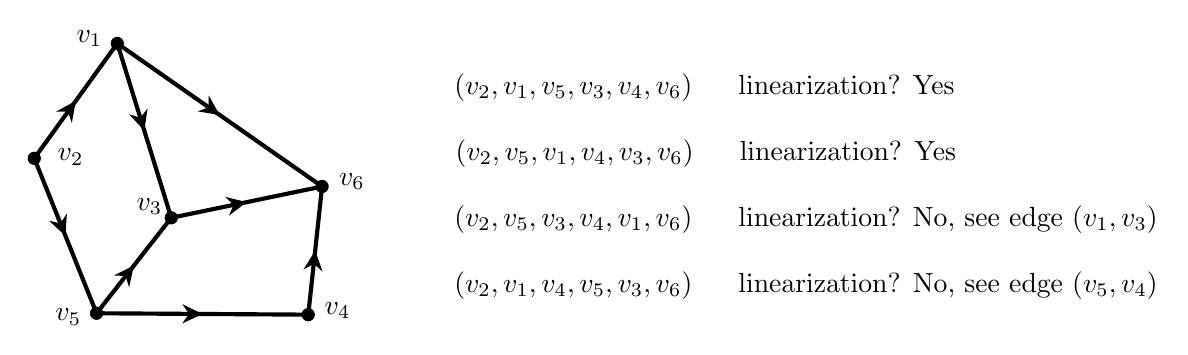
\begin{tikzpicture}[x=0.5pt,y=0.5pt,yscale=-1,xscale=1]
%uncomment if require: \path (0,228); %set diagram left start at 0, and has height of 228

%Flowchart: Connector [id:dp3072392280017706] 
\draw  [fill={rgb, 255:red, 0; green, 0; blue, 0 }  ,fill opacity=1 ] (78,14) .. controls (78,11.58) and (79.96,9.62) .. (82.38,9.62) .. controls (84.79,9.62) and (86.75,11.58) .. (86.75,14) .. controls (86.75,16.42) and (84.79,18.38) .. (82.38,18.38) .. controls (79.96,18.38) and (78,16.42) .. (78,14) -- cycle ;
%Flowchart: Connector [id:dp21397717392367266] 
\draw  [fill={rgb, 255:red, 0; green, 0; blue, 0 }  ,fill opacity=1 ] (63,209) .. controls (63,206.58) and (64.96,204.62) .. (67.38,204.62) .. controls (69.79,204.62) and (71.75,206.58) .. (71.75,209) .. controls (71.75,211.42) and (69.79,213.38) .. (67.38,213.38) .. controls (64.96,213.38) and (63,211.42) .. (63,209) -- cycle ;
%Flowchart: Connector [id:dp8067973087407497] 
\draw  [fill={rgb, 255:red, 0; green, 0; blue, 0 }  ,fill opacity=1 ] (18,97) .. controls (18,94.58) and (19.96,92.62) .. (22.38,92.62) .. controls (24.79,92.62) and (26.75,94.58) .. (26.75,97) .. controls (26.75,99.42) and (24.79,101.38) .. (22.38,101.38) .. controls (19.96,101.38) and (18,99.42) .. (18,97) -- cycle ;
%Flowchart: Connector [id:dp962987276172525] 
\draw  [fill={rgb, 255:red, 0; green, 0; blue, 0 }  ,fill opacity=1 ] (117,140) .. controls (117,137.58) and (118.96,135.62) .. (121.38,135.62) .. controls (123.79,135.62) and (125.75,137.58) .. (125.75,140) .. controls (125.75,142.42) and (123.79,144.38) .. (121.38,144.38) .. controls (118.96,144.38) and (117,142.42) .. (117,140) -- cycle ;
%Straight Lines [id:da5158988833498211] 
\draw [color={rgb, 255:red, 0; green, 0; blue, 0 }  ,draw opacity=1 ][line width=1.5]    (22.38,97) -- (82.38,14) ;
\draw [shift={(52.38,55.5)}, rotate = 125.86] [fill={rgb, 255:red, 0; green, 0; blue, 0 }  ,fill opacity=1 ][line width=0.08]  [draw opacity=0] (14.56,-6.99) -- (0,0) -- (14.56,6.99) -- (9.67,0) -- cycle    ;
%Straight Lines [id:da26521146489140124] 
\draw [color={rgb, 255:red, 0; green, 0; blue, 0 }  ,draw opacity=1 ][line width=1.5]    (67.38,209) -- (121.38,140) ;
\draw [shift={(94.38,174.5)}, rotate = 128.05] [fill={rgb, 255:red, 0; green, 0; blue, 0 }  ,fill opacity=1 ][line width=0.08]  [draw opacity=0] (14.56,-6.99) -- (0,0) -- (14.56,6.99) -- (9.67,0) -- cycle    ;
%Straight Lines [id:da2524996293078703] 
\draw [color={rgb, 255:red, 0; green, 0; blue, 0 }  ,draw opacity=1 ][line width=1.5]    (121.38,140) -- (82.38,14) ;
\draw [shift={(101.88,77)}, rotate = 252.8] [fill={rgb, 255:red, 0; green, 0; blue, 0 }  ,fill opacity=1 ][line width=0.08]  [draw opacity=0] (14.56,-6.99) -- (0,0) -- (14.56,6.99) -- (9.67,0) -- cycle    ;
%Straight Lines [id:da9962026070016303] 
\draw [color={rgb, 255:red, 0; green, 0; blue, 0 }  ,draw opacity=1 ][line width=1.5]    (67.38,209) -- (22.38,97) ;
\draw [shift={(44.88,153)}, rotate = 248.11] [fill={rgb, 255:red, 0; green, 0; blue, 0 }  ,fill opacity=1 ][line width=0.08]  [draw opacity=0] (14.56,-6.99) -- (0,0) -- (14.56,6.99) -- (9.67,0) -- cycle    ;
%Flowchart: Connector [id:dp1566790029206172] 
\draw  [fill={rgb, 255:red, 0; green, 0; blue, 0 }  ,fill opacity=1 ] (216,210) .. controls (216,207.58) and (217.96,205.62) .. (220.38,205.62) .. controls (222.79,205.62) and (224.75,207.58) .. (224.75,210) .. controls (224.75,212.42) and (222.79,214.38) .. (220.38,214.38) .. controls (217.96,214.38) and (216,212.42) .. (216,210) -- cycle ;
%Straight Lines [id:da5810218256695717] 
\draw [color={rgb, 255:red, 0; green, 0; blue, 0 }  ,draw opacity=1 ][line width=1.5]    (67.38,209) -- (220.38,210) ;
\draw [shift={(143.88,209.5)}, rotate = 180.37] [fill={rgb, 255:red, 0; green, 0; blue, 0 }  ,fill opacity=1 ][line width=0.08]  [draw opacity=0] (14.56,-6.99) -- (0,0) -- (14.56,6.99) -- (9.67,0) -- cycle    ;
%Flowchart: Connector [id:dp3466519048019897] 
\draw  [fill={rgb, 255:red, 0; green, 0; blue, 0 }  ,fill opacity=1 ] (226,117.38) .. controls (226,114.96) and (227.96,113) .. (230.38,113) .. controls (232.79,113) and (234.75,114.96) .. (234.75,117.38) .. controls (234.75,119.79) and (232.79,121.75) .. (230.38,121.75) .. controls (227.96,121.75) and (226,119.79) .. (226,117.38) -- cycle ;
%Straight Lines [id:da9047303683615766] 
\draw [color={rgb, 255:red, 0; green, 0; blue, 0 }  ,draw opacity=1 ][line width=1.5]    (121.38,140) -- (230.38,117.38) ;
\draw [shift={(175.88,128.69)}, rotate = 168.27] [fill={rgb, 255:red, 0; green, 0; blue, 0 }  ,fill opacity=1 ][line width=0.08]  [draw opacity=0] (14.56,-6.99) -- (0,0) -- (14.56,6.99) -- (9.67,0) -- cycle    ;
%Straight Lines [id:da5438432067917516] 
\draw [color={rgb, 255:red, 0; green, 0; blue, 0 }  ,draw opacity=1 ][line width=1.5]    (82.38,14) -- (230.38,117.38) ;
\draw [shift={(156.38,65.69)}, rotate = 214.93] [fill={rgb, 255:red, 0; green, 0; blue, 0 }  ,fill opacity=1 ][line width=0.08]  [draw opacity=0] (14.56,-6.99) -- (0,0) -- (14.56,6.99) -- (9.67,0) -- cycle    ;
%Straight Lines [id:da33002644345566856] 
\draw [color={rgb, 255:red, 0; green, 0; blue, 0 }  ,draw opacity=1 ][line width=1.5]    (220.38,210) -- (230.38,117.38) ;
\draw [shift={(225.38,163.69)}, rotate = 96.16] [fill={rgb, 255:red, 0; green, 0; blue, 0 }  ,fill opacity=1 ][line width=0.08]  [draw opacity=0] (14.56,-6.99) -- (0,0) -- (14.56,6.99) -- (9.67,0) -- cycle    ;

% Text Node
\draw (51,3) node [anchor=north west][inner sep=0.75pt]   [align=left] {$\displaystyle v_{1}$};
% Text Node
\draw (94.38,124.38) node [anchor=north west][inner sep=0.75pt]   [align=left] {$\displaystyle v_{3}$};
% Text Node
\draw (35.75,204) node [anchor=north west][inner sep=0.75pt]   [align=left] {$\displaystyle v_{5}$};
% Text Node
\draw (230.38,199.38) node [anchor=north west][inner sep=0.75pt]   [align=left] {$\displaystyle v_{4}$};
% Text Node
\draw (37.38,88.38) node [anchor=north west][inner sep=0.75pt]   [align=left] {$\displaystyle v_{2}$};
% Text Node
\draw (240.75,106.35) node [anchor=north west][inner sep=0.75pt]   [align=left] {$\displaystyle v_{6}$};
% Text Node
\draw (324,34) node [anchor=north west][inner sep=0.75pt]   [align=left] {$\displaystyle ( v_{2} ,v_{1} ,v_{5} ,v_{3} ,v_{4} ,v_{6})$ \ \ \ \ linearization? Yes};
% Text Node
\draw (325,81.67) node [anchor=north west][inner sep=0.75pt]   [align=left] {$\displaystyle ( v_{2} ,v_{5} ,v_{1} ,v_{4} ,v_{3} ,v_{6})$ \ \ \ \ linearization? Yes};
% Text Node
\draw (324,129.34) node [anchor=north west][inner sep=0.75pt]   [align=left] {$\displaystyle ( v_{2} ,v_{5} ,v_{3} ,v_{4} ,v_{1} ,v_{6})$ \ \ \ \ linearization? No, see edge $\displaystyle ( v_{1} ,v_{3})$};
% Text Node
\draw (324,177) node [anchor=north west][inner sep=0.75pt]   [align=left] {$\displaystyle ( v_{2} ,v_{1} ,v_{4} ,v_{5} ,v_{3} ,v_{6})$ \ \ \ \ linearization? No, see edge $\displaystyle ( v_{5} ,v_{4})$};


\end{tikzpicture}

}
\caption{Examples of linearization.}
\end{figure}

If a directed graph $G$ admits a linearization, then we say $G$ can be \emph{linearized}.
We now show that linearization is an \emph{equivalent} characterization of DAGs.

\begin{claim}
A directed graph $G$ can be linearized if and only if $G$ is a DAG.
\label{claim:dag}
\end{claim}

\emph{Proof.}  Let's first prove that if $G$ can be linearized, then $G$ is a DAG.
This is equivalent to proving its contraposition: if $G$ contains a cycle, then $G$ cannot be linearized.
Suppose that there exists an cycle $v_{i_1} \to v_{i_2} \to \cdots \to v_{i_k} \to v_{i_1}$ in $G$.
Then the linearization $X$ must satisfy that $v_{i_{j}}$ is before $v_{i_{j+1}}$ for all $j = 1, 2, \cdots, k-1$,
and that $v_{i_{k}}$ is before $v_{i_1}$, in $X$. Clearly, this is not possible.

The other side of the statement, i.e., if $G$ is a DAG, then $G$ can always be linearized, can be proved constructively.
We will design an algorithm~(see below), that constructs a linearization for any DAG. \qed


